% =============================================================================
% CHƯƠNG 3: THIẾT KẾ MÔ HÌNH MẠNG
% =============================================================================
\chapter{Thiết kế mô hình mạng}

\section{Tổng quan thiết kế}

Mô hình mạng được thiết kế gồm hai phần chính:
\begin{enumerate}
    \item \textbf{Mạng nội bộ (LAN) tại 3 chi nhánh}: Mỗi chi nhánh dùng một kiến trúc LAN khác nhau để so sánh hiệu năng.
    \item \textbf{Backbone Metro Ethernet MPLS của ISP}: Các router CE, PE, P tạo thành hạ tầng kết nối xuyên chi nhánh.
\end{enumerate}

\begin{figure}[H]
    \centering
    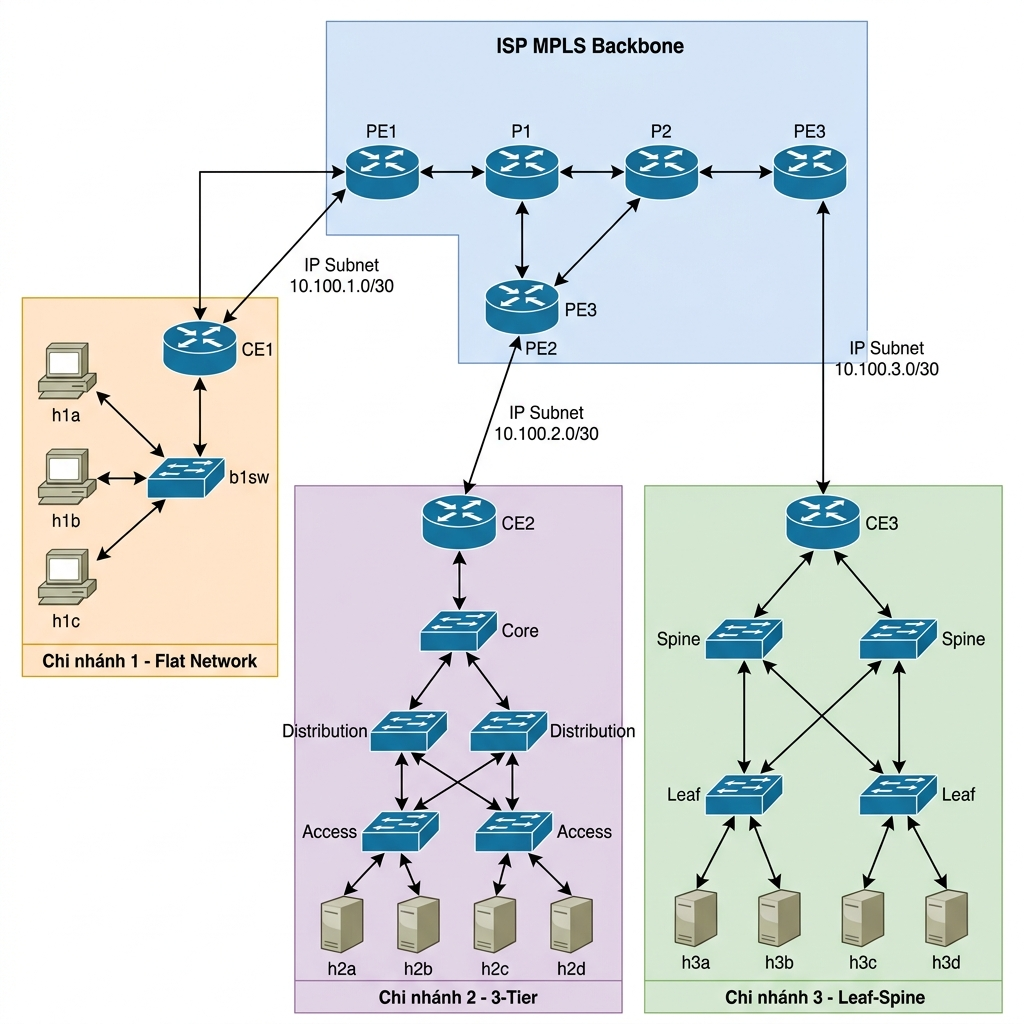
\includegraphics[width=0.95\linewidth]{media/mpls_topology.png}
    \caption{Sơ đồ tổng thể mô hình Metro Ethernet MPLS kết nối 3 chi nhánh}
    \label{fig:mpls_topology}
\end{figure}

\subsection{Sơ đồ logic tổng thể}

\begin{verbatim}
┌─────────────────────────────────────────────────────────────────────┐
│                     ISP METRO ETHERNET MPLS BACKBONE                │
│  ┌──────┐  10.0.12.0/30  ┌──────┐  10.0.99.0/30  ┌──────┐          │
│  │  PE1 │───────────────►│  P1  │◄───────────────►│  P2  │          │
│  │.1   .2                │.2   .1                 │.1   .2│         │
│  └──────┘                └──┬───┘                 └────┬──┘          │
│     │                       │ 10.0.31.0/30             │             │
│     │                  ┌────▼────┐               ┌─────▼────┐        │
│     │                  │   PE3   │               │    PE2   │        │
│     │                  │.1     .2│               │.1      .2│        │
│     │                  └─────────┘               └──────────┘        │
└─────┼──────────────────────┼─────────────────────────┼───────────────┘
      │10.100.1.0/30         │10.100.3.0/30            │10.100.2.0/30
   ┌──▼──┐                ┌──▼──┐                   ┌──▼──┐
   │ CE1 │                │ CE3 │                   │ CE2 │
   └──┬──┘                └──┬──┘                   └──┬──┘
      │10.1.0.0/24           │10.3.0.0/24              │10.2.0.0/24
 ┌────▼────────┐        ┌────▼────────┐          ┌─────▼────────┐
 │ Chi nhánh 1 │        │ Chi nhánh 3 │          │ Chi nhánh 2  │
 │ Flat Network│        │ Leaf-Spine  │          │ 3-Tier (CDA) │
 │ h1a h1b h1c │        │h3a h3b h3c │          │h2a h2b h2c   │
 └─────────────┘        │     h3d    │          │     h2d      │
                        └────────────┘          └──────────────┘
\end{verbatim}

\section{Thiết kế chi nhánh 1: Mạng phẳng (Flat Network)}

\subsection{Cấu trúc topology}

Chi nhánh 1 sử dụng kiến trúc mạng phẳng đơn giản nhất:

\begin{verbatim}
   CE1 (10.1.0.254/24)
    │
   [b1sw – Access Switch Layer 2]
   /│\
h1a h1b h1c
\end{verbatim}

\textbf{Mô tả:}
\begin{itemize}
    \item 1 switch Layer 2 duy nhất (b1sw) kết nối tất cả host.
    \item 3 host: h1a, h1b, h1c – cùng subnet 10.1.0.0/24.
    \item CE1 đóng vai trò default gateway và kết nối lên PE1.
    \item Không có VLAN, không có routing nội bộ – tất cả giao tiếp qua Layer 2.
\end{itemize}

\subsection{Thông số kỹ thuật}
\begin{itemize}
    \item Số switch: 1 (OVS, failMode=standalone)
    \item Số host: 3
    \item Băng thông CE1-PE1: 100 Mbps, delay 5ms
    \item Băng thông host-switch: 100 Mbps
\end{itemize}

\section{Thiết kế chi nhánh 2: Mạng 3 lớp (Core--Distribution--Access)}

\subsection{Cấu trúc topology}

\begin{verbatim}
             CE2 (10.2.0.254/24)
              │
          [b2core – Core Switch]
              │
          [b2dist – Distribution Switch]
             / \
       [b2acc1]  [b2acc2]
        /   \      /   \
      h2a   h2b  h2c   h2d
\end{verbatim}

\textbf{Mô tả:}
\begin{itemize}
    \item \textbf{Access switches} (b2acc1, b2acc2): Kết nối host, mỗi switch 2 host.
    \item \textbf{Distribution switch} (b2dist): Tập hợp uplink từ 2 access switch.
    \item \textbf{Core switch} (b2core): Kết nối distribution lên CE2.
    \item CE2 đóng vai router gateway, kết nối lên PE2.
\end{itemize}

\subsection{Thông số kỹ thuật}
\begin{itemize}
    \item Số switch: 4 (Core × 1 + Dist × 1 + Access × 2)
    \item Số host: 4
    \item Link Access–Distribution: 1 Gbps
    \item Link Distribution–Core: 10 Gbps
    \item Link Core–CE2: 1 Gbps
\end{itemize}

\section{Thiết kế chi nhánh 3: Mạng Leaf-Spine}

\subsection{Cấu trúc topology}

\begin{verbatim}
       CE3 (10.3.0.254/24)
        │
   [b3sp1]─────────[b3sp2]   ← Spine (lõi)
     /  \             /  \
  [b3lf1] ─ ─ ─ ─ [b3lf2]   ← Leaf (truy cập)
   /  \               /  \
 h3a  h3b           h3c  h3d
\end{verbatim}

\textbf{Mô tả:}
\begin{itemize}
    \item 2 \textbf{Spine} switch (b3sp1, b3sp2): Lõi băng thông cao, kết nối full-mesh với mọi Leaf.
    \item 2 \textbf{Leaf} switch (b3lf1, b3lf2): Truy cập host, mỗi Leaf kết nối cả 2 Spine.
    \item Full Mesh Spine-Leaf cho phép ECMP (Equal-Cost Multi-Path).
    \item CE3 kết nối lên Spine1 → PE3.
\end{itemize}

\subsection{Thông số kỹ thuật}
\begin{itemize}
    \item Số switch: 4 (Spine × 2 + Leaf × 2)
    \item Số host: 4
    \item Link Leaf–Spine: 10 Gbps (mỗi Leaf có 2 uplink)
    \item Link inter-Spine: 40 Gbps
    \item Link Leaf–Host: 1 Gbps
\end{itemize}

\section{Thiết kế backbone MPLS của ISP}

\subsection{Topology backbone}

\begin{verbatim}
PE1──────P1──────P2──────PE2
         │
        PE3
\end{verbatim}

\textbf{Mô tả thiết bị:}
\begin{itemize}
    \item \textbf{PE1} (Provider Edge 1): Kết nối CE1 (chi nhánh 1). Push label khi gói vào, Pop khi gói ra.
    \item \textbf{PE2} (Provider Edge 2): Kết nối CE2 (chi nhánh 2).
    \item \textbf{PE3} (Provider Edge 3): Kết nối CE3 (chi nhánh 3).
    \item \textbf{P1} (Provider Core 1): Chỉ Swap label, kết nối PE1, PE3, và P2.
    \item \textbf{P2} (Provider Core 2): Chỉ Swap label, kết nối PE2 và P1.
\end{itemize}

\subsection{MPLS Label Plan}

\begin{table}[htbp]
    \centering
    \caption{Kế hoạch nhãn MPLS (Label Plan)}
    \vspace{0.2cm}
    \begin{tabularx}{\textwidth}{|c|c|>{\raggedright\arraybackslash}X|c|c|c|}
        \hline
        \textbf{LSP} & \textbf{Hướng} & \textbf{Đường đi} & \textbf{Label Push (PE)} & \textbf{Label Swap (P)} & \textbf{Label Pop (PE)} \\ \hline
        LSP-1 & PE1→PE2 & PE1→P1→P2→PE2 & 100 & 100→200 (P1), 200→300 (P2) & pop (PE2) \\ \hline
        LSP-2 & PE1→PE3 & PE1→P1→PE3 & 400 & 400→500 (P1) & pop (PE3) \\ \hline
        LSP-3 & PE2→PE1 & PE2→P2→P1→PE1 & 600 & 600→700 (P2), 700→800 (P1) & pop (PE1) \\ \hline
        LSP-4 & PE2→PE3 & PE2→P2→P1→PE3 & 900 & 900→1000 (P2), 1000→1100 (P1) & pop (PE3) \\ \hline
        LSP-5 & PE3→PE1 & PE3→P1→PE1 & 1200 & 1200→1300 (P1) & pop (PE1) \\ \hline
        LSP-6 & PE3→PE2 & PE3→P1→P2→PE2 & 1400 & 1400→1500 (P1), 1500→1600 (P2) & pop (PE2) \\ \hline
    \end{tabularx}
\end{table}

\section{Bảng địa chỉ IP toàn hệ thống}

\begin{table}[htbp]
    \centering
    \caption{Bảng địa chỉ IP – LAN chi nhánh}
    \vspace{0.2cm}
    \begin{tabularx}{\textwidth}{|c|c|c|c|c|}
        \hline
        \textbf{Chi nhánh} & \textbf{Host} & \textbf{Địa chỉ IP} & \textbf{Subnet} & \textbf{Default GW} \\ \hline
        \multirow{4}{*}{1 – Flat} & h1a & 10.1.0.1 & /24 & 10.1.0.254 \\ \cline{2-5}
                                   & h1b & 10.1.0.2 & /24 & 10.1.0.254 \\ \cline{2-5}
                                   & h1c & 10.1.0.3 & /24 & 10.1.0.254 \\ \cline{2-5}
                                   & CE1-LAN & 10.1.0.254 & /24 & -- \\ \hline
        \multirow{5}{*}{2 – 3-Tier} & h2a & 10.2.0.1 & /24 & 10.2.0.254 \\ \cline{2-5}
                                     & h2b & 10.2.0.2 & /24 & 10.2.0.254 \\ \cline{2-5}
                                     & h2c & 10.2.0.3 & /24 & 10.2.0.254 \\ \cline{2-5}
                                     & h2d & 10.2.0.4 & /24 & 10.2.0.254 \\ \cline{2-5}
                                     & CE2-LAN & 10.2.0.254 & /24 & -- \\ \hline
        \multirow{5}{*}{3 – Leaf-Spine} & h3a & 10.3.0.1 & /24 & 10.3.0.254 \\ \cline{2-5}
                                         & h3b & 10.3.0.2 & /24 & 10.3.0.254 \\ \cline{2-5}
                                         & h3c & 10.3.0.3 & /24 & 10.3.0.254 \\ \cline{2-5}
                                         & h3d & 10.3.0.4 & /24 & 10.3.0.254 \\ \cline{2-5}
                                         & CE3-LAN & 10.3.0.254 & /24 & -- \\ \hline
    \end{tabularx}
\end{table}

\begin{table}[htbp]
    \centering
    \caption{Bảng địa chỉ IP – Backbone ISP MPLS}
    \vspace{0.2cm}
    \begin{tabularx}{\textwidth}{|c|c|c|c|c|}
        \hline
        \textbf{Segment} & \textbf{Interface} & \textbf{Địa chỉ IP} & \textbf{Subnet} & \textbf{Vai trò} \\ \hline
        CE1–PE1 & ce1-wan & 10.100.1.1 & /30 & Customer Edge (Chi nhánh 1) \\ \cline{2-5}
                 & pe1-ce1 & 10.100.1.2 & /30 & Provider Edge (tiếp nhận CE1) \\ \hline
        CE2–PE2 & ce2-wan & 10.100.2.1 & /30 & Customer Edge (Chi nhánh 2) \\ \cline{2-5}
                 & pe2-ce2 & 10.100.2.2 & /30 & Provider Edge (tiếp nhận CE2) \\ \hline
        CE3–PE3 & ce3-wan & 10.100.3.1 & /30 & Customer Edge (Chi nhánh 3) \\ \cline{2-5}
                 & pe3-ce3 & 10.100.3.2 & /30 & Provider Edge (tiếp nhận CE3) \\ \hline
        PE1–P1 & pe1-p1 & 10.0.12.1 & /30 & Provider Edge → Core \\ \cline{2-5}
                & p1-pe1 & 10.0.12.2 & /30 & Core (nhận từ PE1) \\ \hline
        PE2–P2 & pe2-p2 & 10.0.23.1 & /30 & Provider Edge → Core \\ \cline{2-5}
                & p2-pe2 & 10.0.23.2 & /30 & Core (nhận từ PE2) \\ \hline
        PE3–P1 & pe3-p1 & 10.0.31.1 & /30 & Provider Edge → Core \\ \cline{2-5}
                & p1-pe3 & 10.0.31.2 & /30 & Core (nhận từ PE3) \\ \hline
        P1–P2 & p1-p2 & 10.0.99.1 & /30 & Inter-Core Link \\ \cline{2-5}
               & p2-p1 & 10.0.99.2 & /30 & Inter-Core Link \\ \hline
    \end{tabularx}
\end{table}
